\documentclass[10pt,twocolumn]{article}
\usepackage[margin=0.7in]{geometry}
\usepackage{graphicx}
\usepackage{amsmath}
\usepackage{amssymb}
\usepackage{booktabs}
\usepackage{siunitx}
\usepackage[font=small,labelfont=bf]{caption}
\usepackage{xcolor}
\usepackage[colorlinks=true,linkcolor=blue,citecolor=blue,urlcolor=blue]{hyperref}
\graphicspath{{../../results/}}

\setlength{\parskip}{2pt}
\setlength{\parindent}{10pt}

\title{\vspace{-3em}\textbf{netflow}: a generic sparse network solver,\\
demonstrated across thermal, hydraulic, and neutronic physics}
\author{\small greenwoodms06 \quad with Claude (under the Soul System)}
\date{\small 2026--05--20}

\begin{document}
\maketitle

\begin{abstract}
\small
We present \texttt{netflow}, a Python framework that solves problems
reducible to \emph{conservation of a flux at network nodes}. A small,
domain-agnostic core (nodes carrying a scalar state, edges relating two
states to a conserved flux, Newton/Picard solves over
\texttt{scipy.sparse}~\cite{scipy}) hosts physics as plugins. We show the
core is generic not merely across \emph{domains} (thermal, hydraulic,
neutronic) but across \emph{problem structures} (driven boundary-value,
eigenvalue, transient, coupled multiphysics)---all expressed as an
\emph{outer loop of driven core solves}, with no core modifications.
Verification is exact against textbook closed forms. In a \emph{code-to-code}
comparison against published VERA Core Physics Benchmark
solutions~\cite{vera,kelly} (whose Problems~6/7 have no reference
solution), netflow's peak \emph{volume-average} fuel temperature agrees
with the MC21/CTF solution to within 6\%, and its calibrated subchannel
exit-coolant spread brackets the published code spread. A Doppler-coupled
neutronics/thermal solve computes the power self-consistently, exhibiting
the negative temperature feedback that makes reactors stable.
\end{abstract}

\section{Motivation and abstraction}
Many engineering domains share one mathematical skeleton: a quantity is
conserved at the nodes of a network, and each edge carries a flux that
depends on its two endpoint states. Heat conduction (Fourier), pipe flow
(Darcy--Weisbach), neutron diffusion (Fick), and electrical circuits
(Ohm) are all instances. \texttt{netflow} factors this skeleton into a
core with three objects: a \texttt{Node} (scalar state, optional
Dirichlet/Neumann boundary, optional capacitance), an \texttt{Edge}
(\,\texttt{flux}$(s_a,s_b)$ and an optional analytic Jacobian\,), and a
\texttt{Network} that assembles the residual
\begin{equation}
F_i(\mathbf{x}) = \text{source}_i + \!\!\sum_{e=(a,b)}\!\! \big[\,
\mathbb{1}_{b=i}\,f_e - \mathbb{1}_{a=i}\,f_e \,\big] = 0
\end{equation}
and solves it with damped Newton (analytic sparse Jacobian) or a Picard
fallback. The core has \emph{zero} domain imports; a CI ``layering''
test enforces it. Figure~\ref{fig:rosetta} shows the same abstraction
instantiated in four domains.

\begin{figure}[t]
\centering
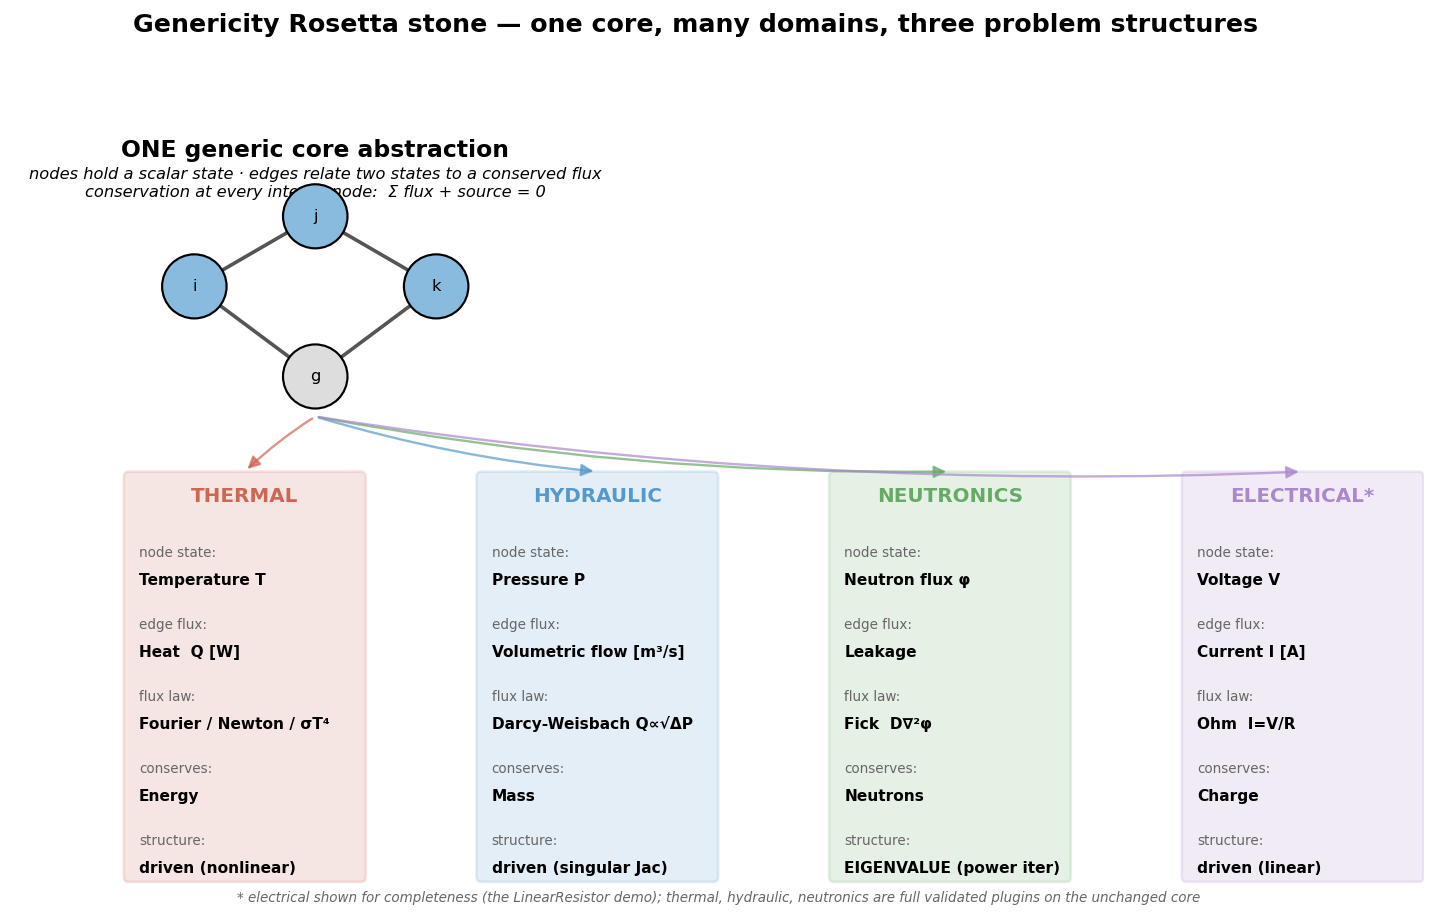
\includegraphics[width=\columnwidth]{rosetta_stone.png}
\caption{One core abstraction across four domains and three problem
structures. State, flux, flux-law, conserved quantity, and mathematical
structure differ; the network solver does not.}
\label{fig:rosetta}
\end{figure}

\section{The meta-abstraction: outer loops}
The core solves \emph{driven} problems $F(\mathbf{x})=0$. Three larger
problem classes reduce to repeated driven solves
(Fig.~\ref{fig:arch}, right):
\begin{itemize}\setlength\itemsep{0pt}
\item \textbf{Transient} ($C_i\,\dot T_i = F_i$): implicit BDF time
stepping~\cite{scipy}; each step is a driven Newton solve. A na\"ive
dense Jacobian costs $\mathcal{O}(N^2)$ memory (15\,GB at a full fuel
assembly); supplying the analytic sparse Jacobian reduces a 7$\times$7
assembly transient from 320\,s to 4.2\,s.
\item \textbf{Eigenvalue} (criticality $M\varphi=k^{-1}P\varphi$): power
iteration, where each step is a driven diffusion solve with the fission
source updated from the previous flux.
\item \textbf{Coupled multiphysics}: Picard iteration between
single-physics solves.
\end{itemize}
All three are captured by one driver,
\texttt{core.iterate.fixed\_point}, on which the power-iteration solver
is built. This is the framework's central finding: genericity across
problem \emph{structure}, achieved by composition rather than by
special-casing the core.

\begin{figure}[t]
\centering
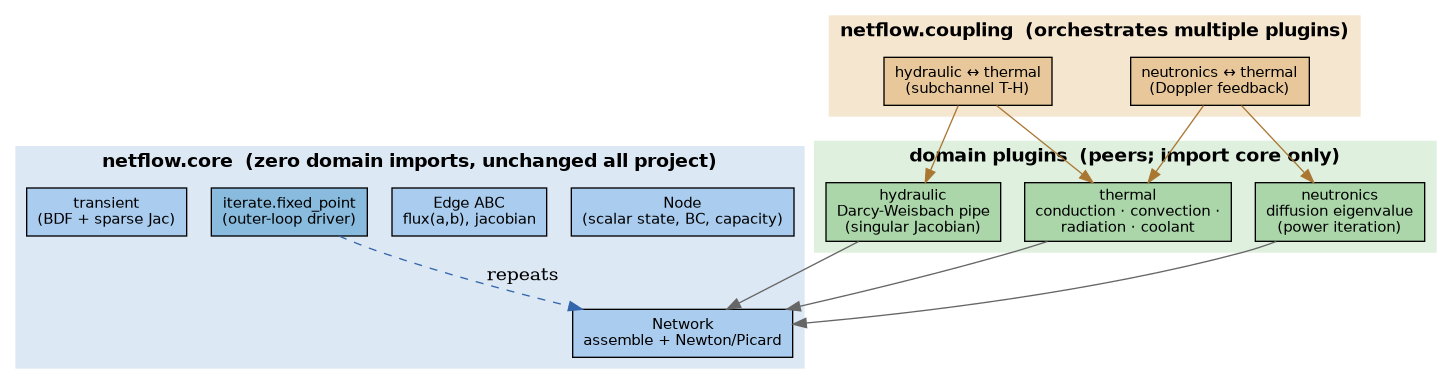
\includegraphics[width=\columnwidth]{arch_diagram.png}
\caption{Layered architecture. The core (blue, unchanged for the entire
project) is wrapped by peer domain plugins (green) and a coupling layer
(orange) that orchestrates several plugins. Plugins never import each
other; coupling code may.}
\label{fig:arch}
\end{figure}

\section{Verification}
Each edge is checked against its analytic resistance; analytic Jacobians
agree with finite differences to $\le10^{-5}$. The thermal fuel-pin
chain reproduces the textbook radial decomposition (film, gap, clad,
fuel)~\cite{todreas} to machine precision. Neutron-diffusion $k$-eff
converges to the analytic bare-slab value as
$\mathcal{O}(\Delta^2)$---9.7, 1.5, 0.4, 0.1\,pcm at $N=20,50,100,200$
cells---with the fundamental mode matching the analytic cosine exactly.
Global energy balance on a full assembly closes to six significant
figures. The suite is 107 automated tests.

\section{Code-to-code comparison against VERA}
We match the VERA Watts~Bar 17$\times$17 geometry~\cite{vera} exactly.
The benchmark's Problems~6/7 \emph{define inputs only}---the
specification states ``no reference solution exists''~\cite{vera}---so
published P6/P7 results are themselves code solutions, and this is
honestly a code-to-code comparison, not validation against a reference
truth. Compared \emph{at the published definition} (VERA reports
\emph{volume-average}, not centerline, fuel temperature), netflow's peak
volume-average fuel temperature is \SI{999}{\celsius} against the
MC21/CTF value of \SI{1066}{\celsius}~\cite{kelly} ($-6\%$), for a single
hot pin at matched local peaking ($1.918$ vs.\ the published $1.92$),
using the empirical gap conductance (a controlled comparison showed a
geometric helium-gap model over-predicts by ${\sim}220$\,K). The coolant
mean rise (\SIrange{37}{39}{K}) matches the assembly energy balance
(${\sim}\SI{36}{K}$). Subchannel exit-coolant spread is a
\emph{calibrated} quantity in any scalar model: for the near-flat
Problem~6 power, sweeping the lateral-mixing fraction over $0.05$--$0.40$
gives \SIrange{4.9}{6.5}{K}, essentially matching the published
\SI{6.6}{K} (MC21/CTF, VERA) and under \SI{8.7}{K}
(MC21/COBRA-IE)~\cite{aviles}, with guide tubes appearing as cool bypass
channels as in the benchmark. The mixing coefficient is calibrated, not
predicted: \texttt{netflow} is a transparent pre-design tool, not a
replacement for CTF/COBRA-TF.

\begin{table}[t]
\centering\small
\caption{netflow vs published VERA P6/P7 code solutions~\cite{kelly,aviles}
(code comparison --- P6/P7 have no reference solution).}
\label{tab:introcompare}
\begin{tabular}{lcc}
\toprule
quantity & netflow & published \\
\midrule
peak vol-avg fuel T (\si{\celsius}) & 999 & 1066 \\
coolant exit spread (\si{K}) & 4.9--6.5 & 6.6\,/\,8.7 \\
coolant mean rise (\si{K}) & 37--39 & 34--37 \\
$k$ convergence (verification) & $\le$0.1\,pcm & analytic \\
\bottomrule
\end{tabular}
\end{table}

\begin{figure}[t]
\centering
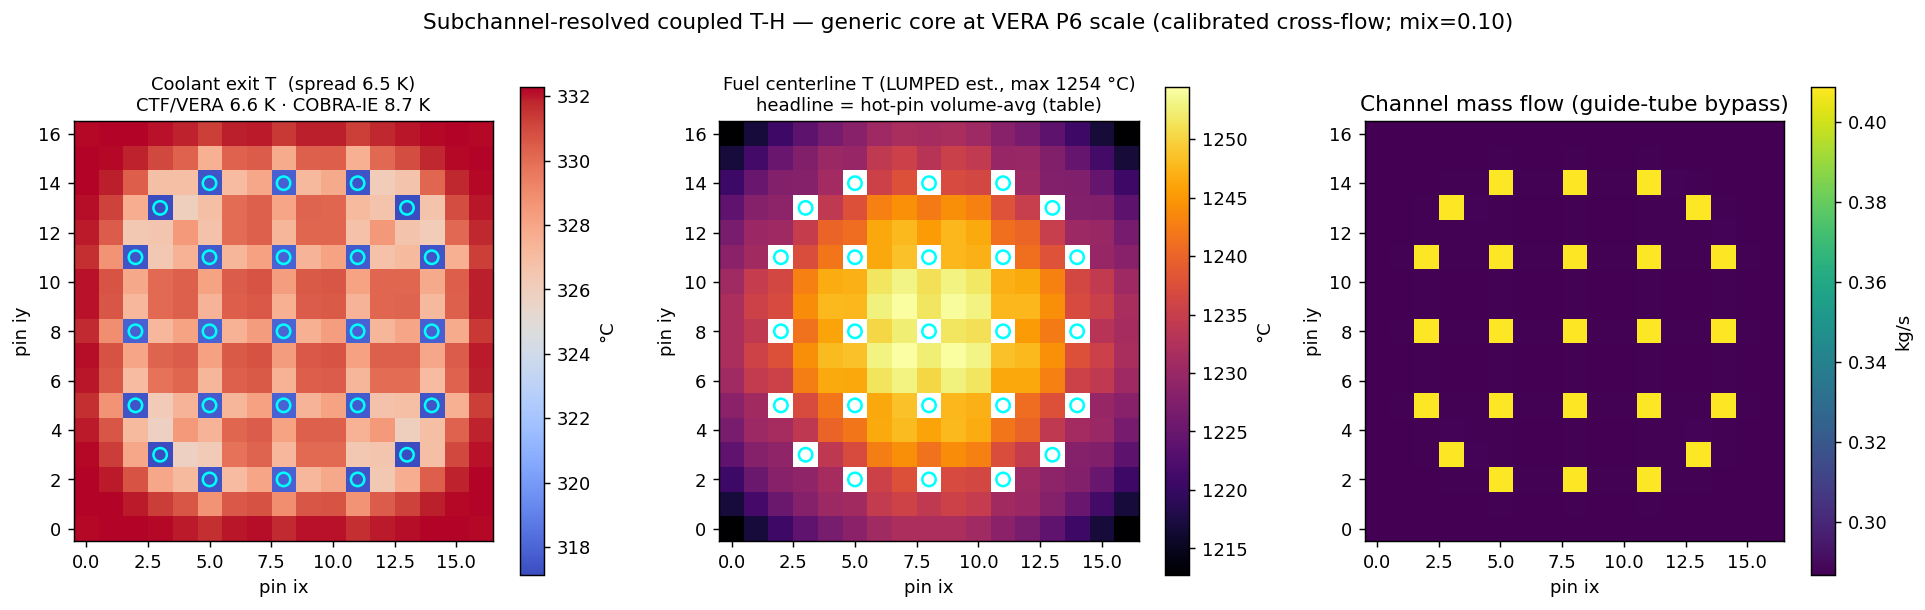
\includegraphics[width=\columnwidth]{subchannel_pinresolved.png}
\caption{Pin-resolved subchannel coupled thermal--hydraulics
(17$\times$17). Left: coolant exit temperature---guide tubes (cyan) form
cool spots, matching the VERA pattern. Right: guide-tube bypass flow.}
\label{fig:subch}
\end{figure}

\section{Self-consistent multiphysics}
Coupling the neutronics and thermal plugins through Picard iteration,
with Doppler feedback ($\Sigma_a\!\propto\!\sqrt{T}$), \emph{computes}
the power distribution rather than imposing it---closing the central
caveat of the temperature comparisons. The coupled solve exhibits a
\emph{negative} fuel-temperature reactivity coefficient
(Fig.~\ref{fig:doppler})---the sign underlying inherent reactor
stability---and the flux Doppler-flattens at power. We report this as a
mechanism/sign demonstration only: it runs on a one-group bare slab with
illustrative cross-sections, so its magnitude is not a physical
prediction. The physical reference for fresh 3.10\,wt\%
UO\textsubscript{2}, $-2$ to $-2.5$\,pcm/K, is itself derived from the
spec's reference KENO-VI eigenvalues for Problems~1--2~\cite{vera}.

\begin{figure}[t]
\centering
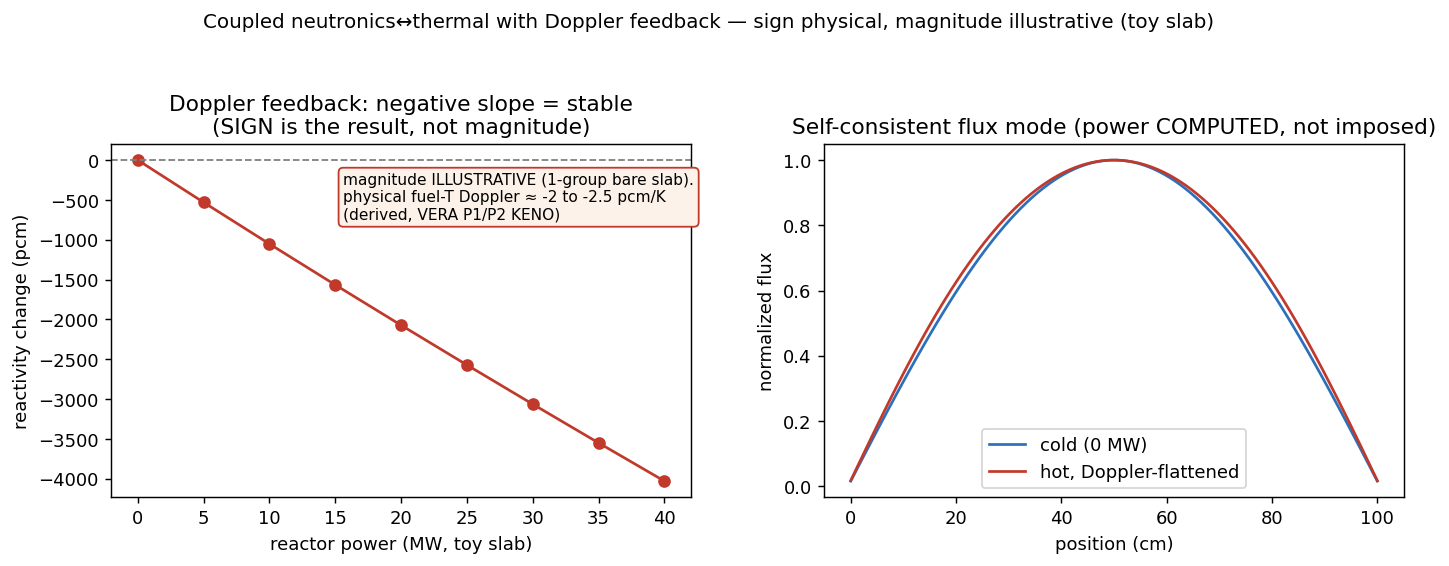
\includegraphics[width=\columnwidth]{doppler_feedback.png}
\caption{Doppler-coupled neutronics/thermal. Left: reactivity vs.\ power
(negative slope $=$ stable) --- the \emph{sign} is the result; the toy-slab
magnitude is illustrative (physical $\approx -2$ to $-2.5$\,pcm/K). Right: the
self-consistent flux mode flattens at power. Power is computed, not imposed.}
\label{fig:doppler}
\end{figure}

\section{Performance and scope}
Solve time is linear in node count until sparse-factorization fill-in
dominates near $4\times10^5$ unknowns ($\sim$190\,s for a 1/8-core
slice); Newton iteration count is invariant with size. The identified
limits---gap-conductance fidelity, subchannel momentum closure, and the
$\sim$$10^6$-node factorization wall---are documented as deliberate
future work, not hidden. \texttt{netflow} targets fast, transparent
pre-design scoping accurate to tens of $^\circ$C, cross-checked against
published benchmark code solutions, on a single core that also solves pipe
networks and criticality problems. netflow's node/edge/flux abstraction is
the acausal across/through-variable connector of Modelica~\cite{modelica}
and ModelingToolkit~\cite{mtk}; it is a minimal, transparent, pure-Python
re-derivation of that mature paradigm, not a new one nor a replacement for
those tools.

\begin{thebibliography}{9}\small
\bibitem{vera} A.~T.~Godfrey, \emph{VERA Core Physics Benchmark
Progression Problem Specifications}, CASL-U-2012-0131-004, Oak Ridge
National Laboratory, 2014.
\bibitem{kelly} D.~J.~Kelly III \emph{et al.}, ``MC21/CTF and VERA
multiphysics solutions to VERA core physics benchmark progression
problems 6 and 7,'' \emph{Nucl.\ Eng.\ Technol.} \textbf{49} (2017)
1326--1338.
\bibitem{aviles} B.~N.~Aviles \emph{et al.}, ``MC21/COBRA-IE and
VERA-CS multiphysics solutions to VERA core physics benchmark problem
\#6,'' \emph{Prog.\ Nucl.\ Energy} \textbf{101} (2017) 338--351.
\bibitem{todreas} N.~E.~Todreas and M.~S.~Kazimi, \emph{Nuclear Systems
I: Thermal Hydraulic Fundamentals}, 2nd ed., CRC Press, 2012.
\bibitem{scipy} P.~Virtanen \emph{et al.}, ``SciPy 1.0: fundamental
algorithms for scientific computing in Python,'' \emph{Nature Methods}
\textbf{17} (2020) 261--272.
\bibitem{coolprop} I.~H.~Bell \emph{et al.}, ``Pure and pseudo-pure fluid
thermophysical property evaluation and the open-source thermophysical
property library CoolProp,'' \emph{Ind.\ Eng.\ Chem.\ Res.} \textbf{53}
(2014) 2498--2508.
\bibitem{modelica} Modelica Association, \emph{Modelica Language
Specification}; P.~Fritzson, \emph{Principles of Object-Oriented Modeling
and Simulation with Modelica}, 2nd ed., Wiley, 2014.
\bibitem{mtk} Y.~Ma \emph{et al.}, ``ModelingToolkit: A Composable Graph
Transformation System for Equation-Based Modeling,'' arXiv:2103.05244 (2021).
\end{thebibliography}

\end{document}
